% Concise English synthesis of the supplied thesis, not a full translation.
% Compile twice with pdfLaTeX from this directory. Figures are unchanged originals.
\documentclass[11pt,a4paper]{article}
\usepackage[margin=22mm,headheight=14pt,headsep=7mm,footskip=10mm]{geometry}
\usepackage[T1]{fontenc}
\usepackage{lmodern,amsmath,amssymb,booktabs,array,graphicx,xcolor}
\usepackage{tikz}
\usetikzlibrary{arrows.meta,positioning}
\usepackage{caption,fancyhdr,hyperref}
\definecolor{navy}{HTML}{183247}
\definecolor{teal}{HTML}{006C75}
\definecolor{muted}{HTML}{52626C}
\hypersetup{colorlinks=true,linkcolor=teal,urlcolor=teal,citecolor=teal,
  pdftitle={Energy-Based Swing-Up and Local Stabilization of a Cart-Pendulum},
  pdfauthor={Ali Ramezanzadeh},pdfsubject={Concise English thesis report}}
\captionsetup{font=small,labelfont=bf,skip=5pt,hypcap=false}
\setlength{\parindent}{0pt}
\setlength{\parskip}{6pt}
\renewcommand{\arraystretch}{1.15}
\linespread{1.04}
\pagestyle{fancy}
\fancyhf{}
\fancyhead[L]{\small\color{muted}Cart--pendulum energy-based control}
\fancyhead[R]{\small\color{muted}Ali Ramezanzadeh}
\fancyfoot[C]{\small\thepage\ / 10}
\renewcommand{\headrulewidth}{0.3pt}
\newcommand{\reportsection}[1]{\section*{\color{navy}#1}}
\newcommand{\topic}[1]{\subsection*{\color{teal}#1}}
\newcommand{\qref}{x^{\star}}
\newcommand{\fig}[3]{\begin{center}\includegraphics[width=\linewidth,height=#2,keepaspectratio]{figures/#1}\captionof{figure}{#3}\end{center}}
\newcommand{\note}[1]{\begin{quote}\small\color{muted}#1\end{quote}}
\begin{document}

% PAGE 1
\thispagestyle{plain}
{\small\sffamily\color{teal}NONLINEAR CONTROL\quad /\quad CONCISE THESIS REPORT}
\vspace{8mm}

{\fontsize{26}{30}\selectfont\bfseries\color{navy}
Energy-Based Swing-Up\par
and Local Stabilization\par
of a Cart--Pendulum\par}
\vspace{4mm}
{\large\color{muted}Energy shaping, IDA-PBC, and smooth controller blending}

\vspace{6mm}
{\Large\bfseries Ali Ramezanzadeh}\par
Department of Electrical Engineering, Amirkabir University of Technology\par
Supervisors: Dr. Heidar Ali Talebi and Dr. Iman Sharifi\par
Original thesis date: February 2026\par
English synthesis: October 2026

\reportsection{Abstract}
This report summarizes a thesis study of energy-based control for an underactuated cart--pendulum. The objective is to bring the pendulum toward its unstable upright equilibrium while regulating cart position. Partial feedback linearization produces an acceleration-input model. An energy regulator drives the pendulum toward the upright energy level, and an interconnection and damping assignment passivity-based control (IDA-PBC) implementation provides local regulation. A cubic smoothstep blends the two controller commands within an angular transition band; the auxiliary command is clipped to a prescribed interval.

The supplied MATLAB/Simulink figures document three scenarios: local stabilization, swing-up followed by regulation, and recovery after finite-duration disturbances. These recorded trajectories approach the desired upright configuration and cart reference. The disturbance test also exhibits substantial cart travel and temporary return to swing-up control after the largest pulse.

The study demonstrates the intended control sequence for the illustrated nominal simulations. Its evidence consists of the original thesis, saved models, Live Script, and exported figures; the simulations were not rerun for this synthesis. Inspection identifies differences in coordinate conventions, initial-velocity ordering, and shaped-energy calculations. Consequently, the report distinguishes the established IDA-PBC design framework from the implemented candidate and does not claim a verified global stability guarantee under blending, saturation, and disturbances. The accompanying repository preserves the original files and documents the checks needed for exact reproduction.

\vspace{2mm}
\textbf{Keywords:} underactuated systems; cart--pendulum; energy shaping; IDA-PBC; nonlinear control; MATLAB/Simulink.
\note{This is a selective English technical synthesis, with retained original simulation figures. It is not a full translation, a new experimental study, or a peer-reviewed publication.}

\clearpage
% PAGE 2
\reportsection{1. Mechanical model and input coordinates}
\topic{System and convention}
The cart has mass $M$ and horizontal position $x$. A point mass $m$ is attached to a massless rod of length $l$. Let $\theta=0$ denote the upright position and take the positive angle toward positive cart displacement, so that the pendulum mass has coordinates
\[
 X=x+l\sin\theta,\qquad Y=l\cos\theta.
\]
This convention is consistent with the negative input coupling in the saved reduced model. The manuscript's initial geometric derivation uses the opposite angle direction; the equations below use one convention throughout.

\begin{center}
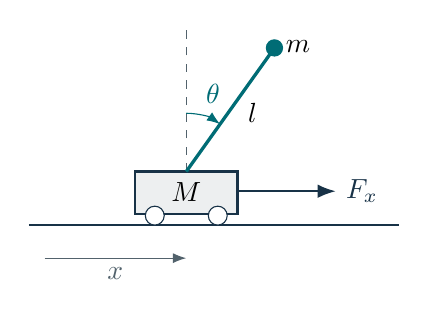
\begin{tikzpicture}[scale=1,>=Latex]
 \draw[thick,navy] (-2,0)--(2.7,0);
 \draw[fill=navy!8,draw=navy,thick] (-.65,.14) rectangle (.65,.68);
 \draw[fill=white,draw=navy] (-.4,.12) circle (.12);
 \draw[fill=white,draw=navy] (.4,.12) circle (.12);
 \draw[dashed,muted] (0,.68)--(0,2.5);
 \draw[very thick,teal] (0,.68)--(1.12,2.25);
 \fill[teal] (1.12,2.25) circle (.11);
 \draw[->,teal] (0,1.42) arc (90:54.5:.74);
 \node[teal] at (.34,1.67) {$\theta$};
 \node at (.84,1.43) {$l$};
 \node at (1.42,2.27) {$m$};
 \node at (0,.42) {$M$};
 \draw[->,navy,thick] (.65,.43)--(1.9,.43) node[right] {$F_x$};
 \draw[->,muted] (-1.8,-.42)--(0,-.42) node[midway,below] {$x$};
\end{tikzpicture}
\captionof{figure}{Cart--pendulum geometry under the convention adopted in this report. The force acts on the cart; the pendulum joint is unactuated.}
\end{center}

\topic{Dynamics and partial feedback linearization}
The kinetic and potential energies are
\begin{align}
 T&=\tfrac12(M+m)\dot x^2+ml\cos\theta\,\dot x\dot\theta+\tfrac12ml^2\dot\theta^2,\\
 V&=mgl\cos\theta.
\end{align}
The Euler--Lagrange equations give
\begin{align}
 (M+m)\ddot x+ml\cos\theta\,\ddot\theta-ml\sin\theta\,\dot\theta^2&=F_x,\\
 l\ddot\theta+\cos\theta\,\ddot x-g\sin\theta&=0.
\end{align}
With the auxiliary input $u=\ddot x$, define $a=g/l$ and $b=1/l$. Then
\begin{equation}\label{eq:reduced}
 \ddot\theta=a\sin\theta-b\cos\theta\,u,\qquad\ddot x=u.
\end{equation}
For this convention, the equivalent physical force is
\begin{equation}
 F_x=(M+m\sin^2\theta)u+mg\sin\theta\cos\theta-ml\sin\theta\,\dot\theta^2.
\end{equation}
The saved model evolves the reduced dynamics directly. Its separate force-conversion branch uses the opposite angle convention and feeds diagnostics rather than a physical-force plant. Reconciliation is needed before interpreting that force trace quantitatively. An auxiliary acceleration limit does not establish a motor-force limit.

\clearpage
% PAGE 3
\reportsection{2. Energy regulation for swing-up}
\topic{Energy target}
For the angular subsystem, let $\omega=\dot\theta$ and $I=ml^2$. Choose a gravitational reference at the downward position:
\begin{equation}
 H_s(\theta,\omega)=\tfrac12 I\omega^2+mgl(1+\cos\theta),
 \qquad H_s^{\star}=2mgl.
\end{equation}
The error $E=H_s-H_s^{\star}$ is zero at the upright rest configuration. It is negative at downward rest, where $E=-2mgl$. This angular energy is distinct from the total physical cart--pendulum energy, which also contains cart kinetic energy and velocity coupling.

Using \eqref{eq:reduced} and $Ia=mgl$, differentiation yields
\begin{equation}
 \dot E=-Ib\,\omega\cos\theta\,u.
\end{equation}
The energy-pumping component of the project controller is
\begin{equation}
 u_{\rm pump}=k_E E\omega\cos\theta,\qquad k_E>0.
\end{equation}
For $W=\tfrac12E^2$, the ideal, unsaturated energy-only feedback gives
\begin{equation}\label{eq:energydecay}
 \dot W=-Ib k_E E^2\omega^2\cos^2\theta\leq0.
\end{equation}
Energy regulation is a useful swing-up principle: it changes the oscillation amplitude by controlling the energy level rather than tracking a prescribed angle trajectory. The thesis adopts this general idea, associated with the cart--pendulum energy-control literature \cite{chung,thesis}.

\topic{Cart feedback and the implemented objective}
The final swing-up command adds cart-position and cart-velocity feedback:
\begin{equation}\label{eq:swing}
 u_E=k_E E\omega\cos\theta-k_x(x-\qref)-k_v\dot x.
\end{equation}
The reported gains are $k_E=0.9$, $k_x=0.5$, and $k_v=0.1$. The last two terms oppose cart displacement and velocity; the desired cart position is $\qref$. They introduce additional terms into the derivative of $W$, so \eqref{eq:energydecay} is not, by itself, a stability proof for the complete controller.

An energy level is a set of states rather than a unique equilibrium. In particular, $E=0$ can hold away from $(\theta,\omega)=(0,0)$. Swing-up must therefore be followed by a local regulating controller. At exact downward rest with zero cart error and velocity, every term in \eqref{eq:swing} vanishes. An initial perturbation or explicit start-up action may be needed; the recorded swing-up scenarios already contain nonzero initial velocities.

\topic{Design interpretation}
The energy gain controls the strength of pumping. The cart terms influence travel and transient motion. Stronger pumping does not automatically mean a more feasible motion: it can increase saturation and cart excursion. The supplied results should be read as demonstrations at selected gains, rather than an optimization study or a measured region of attraction.

\clearpage
% PAGE 4
\reportsection{3. IDA-PBC framework and energy candidate}
IDA-PBC assigns a desired closed-loop energy and interconnection/damping structure. Under valid matching conditions, the desired energy can serve as a Lyapunov function \cite{ortega,acosta}. For the auxiliary model, write
\[
 q=\begin{bmatrix}\theta\\x\end{bmatrix},\quad
 p=\dot q,\quad
 G(q)=\begin{bmatrix}-b\cos\theta\\1\end{bmatrix},\quad
 H=\tfrac12p^Tp+a\cos\theta.
\]
Here $p$ denotes coordinate velocities in the reduced model, not physical mechanical momenta. A desired energy is
\begin{equation}\label{eq:Hd}
 H_d(q,p)=\tfrac12p^TM_d^{-1}(\theta)p+V_d(q).
\end{equation}
The thesis studies the following inertia parameterization, with $c=\cos\theta$:
\begin{equation}
 M_d(\theta)=\begin{bmatrix}
 \frac{kb^2}{3}c^3&-\frac{kb}{2}c^2\\
 -\frac{kb}{2}c^2&k(c-1)+m_0
 \end{bmatrix},\qquad m_0=m_{22}^0.
\end{equation}
Its determinant is
\begin{equation}
 \det M_d=\frac{kb^2c^3}{12}\big[4(m_0-k)+kc\big].
\end{equation}
The manuscript gives $m_0>k$ as a sufficient condition on the upper half-plane. The chosen $m_0=k=0.2$ also gives positive definiteness wherever $c>0$, since then $\det M_d=k^2b^2c^4/12>0$. The matrix becomes singular at the boundary $\lvert\theta\rvert=\pi/2$.

\topic{Potential shaping and controller structure}
The printed energy candidate uses
\begin{align}
 V_d(q)&=\frac{3a}{kb^2\cos^2\theta}+\frac{P}{2}z(q)^2,\\
 z(q)&=x-\qref+\frac{3}{b}\ln(\sec\theta+\tan\theta)
                 +\frac{6m_0}{kb}\tan\theta.
\end{align}
It has a strict local minimum at $(\theta,x)=(0,\qref)$ for positive $a,k,P$. A minimum alone does not establish matching with the plant. This distinction matters because inspection found inconsistencies between the printed matching formulas and the implementation, discussed in Section 8.

With $G^\dagger=(G^TG)^{-1}G^T$ and $R_2=GK_vG^T$, the project uses the controller structure
\begin{equation}
 u_S=G^\dagger\big[\nabla_q V-M_d\nabla_q H_d-R_2M_d^{-1}p\big].
\end{equation}
Its implementation omits a gyroscopic term. In an exactly matched desired system, damping would yield $\dot H_d=-K_v(G^TM_d^{-1}p)^2\leq0$; convergence would additionally require an invariance/detectability argument. These conditions have not been independently established for the saved controller, so this report treats it as an IDA-PBC-inspired implementation.

\clearpage
% PAGE 5
\reportsection{4. Smooth blending and simulation setup}
\topic{Angular transfer rule}
Let $d=\lvert\theta\rvert$, $\varepsilon=\pi/2-0.9$, and $d_1=\varepsilon-\delta$, $d_2=\varepsilon+\delta$. For $\tau=(d-d_1)/(d_2-d_1)$, the active weighting rule is
\begin{equation}
 \alpha(d)=\begin{cases}
 1,&d\leq d_1,\\
 1-3\tau^2+2\tau^3,&d_1<d<d_2,\\
 0,&d\geq d_2.
 \end{cases}
\end{equation}
The saved model uses $\delta=0.03$ rad. The overview image contains $0.07$ instead; it represents a different setting. The active transition depends on angle, without a velocity gate or dwell-time condition. A continuous weight reduces switching discontinuities but does not prove stability of the blend or prevent command peaks.
\begin{equation}
 u=\operatorname{sat}_{[-10,10]}\!\left[(1-\alpha)u_E+\alpha u_S\right].
\end{equation}

\begin{center}
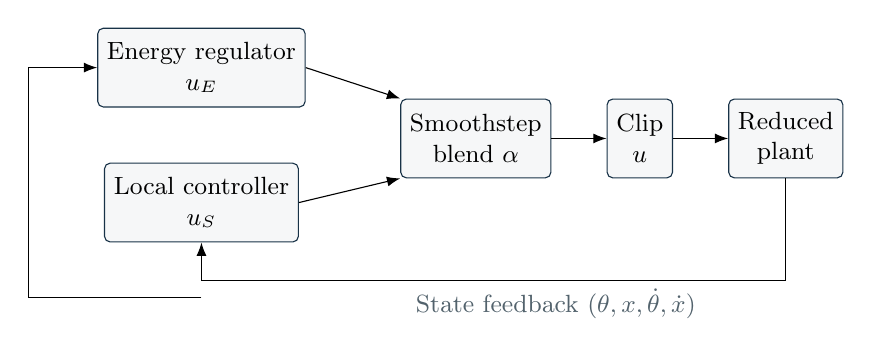
\begin{tikzpicture}[>=Latex,box/.style={draw=navy,rounded corners=2pt,fill=navy!4,align=center,font=\small,minimum height=10mm},node distance=7mm]
 \node[box] (e) {Energy regulator\\$u_E$};
 \node[box,below=of e] (s) {Local controller\\$u_S$};
 \node[box,right=12mm of e,yshift=-9mm] (blend) {Smoothstep\\blend $\alpha$};
 \node[box,right=of blend] (sat) {Clip\\$u$};
 \node[box,right=of sat] (plant) {Reduced\\plant};
 \draw[->] (e.east)--(blend.north west);
 \draw[->] (s.east)--(blend.south west);
 \draw[->] (blend)--(sat);
 \draw[->] (sat)--(plant);
 \draw[->] (plant.south)--++(0,-13mm)-|(s.south);
 \draw[->] (s.south)++(0,-7mm)--++(-22mm,0)|-(e.west);
 \node[font=\small,color=muted] at (4.5,-3.0) {State feedback $(\theta,x,\dot\theta,\dot x)$};
\end{tikzpicture}
\captionof{figure}{Control architecture of the active reduced-coordinate simulation. Disturbances enter the plant; equivalent force is computed separately for inspection.}
\end{center}

\begin{center}\small
\begin{tabular}{@{}p{76mm}p{70mm}@{}}
\toprule
Quantity & Value / recorded setting\\\midrule
Cart / pendulum mass & $M=1$ kg / $m=0.1$ kg\\
Rod length / gravity & $l=0.5$ m / $g=9.81$ m s$^{-2}$\\
Reduced coefficients & $a=19.62$, $b=2$\\
Swing-up gains & $k_E=0.9$, $k_x=0.5$, $k_v=0.1$\\
Local design gains & $k=m_0=0.2$, $K_v=1$, $P=7$\\
Auxiliary command interval & $[-10,10]$ m s$^{-2}$\\
Saved model release & MATLAB/Simulink R2022b\\
Saved integration settings & FixedStepAuto; step $0.001$ s; stop $50$ s\\\bottomrule
\end{tabular}
\captionof{table}{Physical and controller parameters, together with settings read from the saved models. These settings do not independently prove how each historical figure was generated.}
\end{center}

The Live Script contains symbolic modeling, an LQR calculation, potential-surface studies, and plotting from an existing simulation output. Its $P=10$ surface-study setting differs from the local controller's $P=7$. It is not a complete script that recreates all three reported scenarios in one run.

\clearpage
% PAGE 6
\reportsection{5. Recorded local stabilization}
The first scenario starts within the upper half-plane and tests local regulation toward $\theta=0$, $x=0$. The manuscript reports initial coordinates $q(0)=[\pi/2-1,-0.5]^T$. It lists $p(0)=[0.2,-0.2]^T$, while the plotted angular and cart velocities start near $-0.2$ and $0.2$, respectively. Inspection of the saved model confirms that its initial-value labels route the two velocity components in this reversed order. This should be reconciled before an exact replay.

\fig{local-states.png}{75mm}{Original local-stabilization traces over the displayed 0--10 s interval. Panels show $\theta$, $\dot\theta$, $x$, and $\dot x$; model units are rad, rad s$^{-1}$, m, and m s$^{-1}$. The original axes omit explicit unit labels.}

The angle exhibits a damped transient toward upright. The cart moves from its negative initial position, makes a positive excursion, and returns toward its zero reference more slowly. The two velocity traces approach zero. These observations support local regulation for this recorded trajectory, without defining a numerical settling tolerance or a tested region of attraction.

\fig{local-energy.png}{57mm}{Original diagnostic labelled $H_d$. The trace decreases overall with transient rises; it is not monotonically decreasing. Its implementation differs from the inverse-inertia energy in \eqref{eq:Hd}.}

The energy diagnostic is useful as a visualization of the transient, but it must not be used as an independently verified Lyapunov trace. The recorded input figure, retained in the original-source directory, also shows a brief encounter with the positive auxiliary saturation limit. Thus, local convergence in this example does not imply that the controller operated entirely without clipping.

\clearpage
% PAGE 7
\reportsection{6. Recorded swing-up and controller transfer}
The second scenario starts at the downward angle, with initial cart position $x(0)=1$ and reference $\qref=2$. The thesis lists $p(0)=[1,-1.5]^T$; the displayed curves instead begin at angular velocity approximately $-1.5$ and cart velocity approximately $1$. As in the local case, the source velocity order must be interpreted through the model routing.

\fig{swingup-states.png}{72mm}{Original 0--20 s swing-up response. Passages across $\pm\pi$ produce jumps in the wrapped angle display; they do not represent instantaneous physical angular jumps. The cart approaches its reference after the swing-up transient.}

\fig{swingup-inputs.png}{62mm}{Original auxiliary command (blue) and reconstructed-force diagnostic (red dashed). They have different units; the force branch also uses a different sign convention. The auxiliary command reaches its positive clipping limit near transfer.}

Repeated oscillations precede capture near upright. The thesis reports a trigger near $5.54$ s and a transition of roughly $50$ ms; its transfer close-up is retained in the repository. These are approximate historical timings, with smoothing-width differences between the saved model and overview still unresolved. The recorded response illustrates successful transfer for one initial condition. Continuous weighting coexists with saturation and does not establish a small command derivative or guaranteed capture for all upper-half-plane states.

\clearpage
% PAGE 8
\reportsection{7. Recorded disturbance recovery}
The third scenario tests recovery during a $50$ s display window. The initial angle is downward, the initial cart position is $1$, and the cart reference is $2$. The text lists $p(0)=[0.2,-0.4]^T$. The saved model routes these labels to cart velocity $0.2$ and angular velocity $-0.4$, consistent with the displayed curves.

\begin{center}
\begin{tabular}{@{}ccc@{}}
\toprule
Pulse & Time interval (s) & Cart acceleration (m s$^{-2}$)\\\midrule
1 & 10--10.5 & $+3$\\
2 & 15--16 & $+5$\\
3 & 20--20.5 & $-12$\\\bottomrule
\end{tabular}
\captionof{table}{Finite-duration pulses from the saved disturbance function, consistent with the original pulse figure retained in the repository. They enter cart acceleration after command clipping; they are not motor-force pulses or Dirac impulses.}
\end{center}

\fig{disturbance-states.png}{75mm}{Original disturbed response over 0--50 s. Upright and cart-reference regulation recover after the pulse sequence. The largest disturbance produces renewed wrapped-angle passages and a substantial cart excursion.}

The first two pulses perturb the stabilized response without a prolonged return to swing-up. Following the largest negative pulse, the switching record shows temporary re-entry to swing-up, with more than one transition before local regulation is restored. Both command limits are reached during the recovery transient.

The cart-position curve travels below $-6$ on the original scale before returning toward $2$. This large excursion is an essential qualification: the simulation contains no demonstrated finite-rail constraint, and the plotted recovery cannot be treated as evidence that a laboratory cart would remain within a physical travel range. Because the disturbance is added after clipping, total cart acceleration is not restricted to the command's $[-10,10]$ interval.

The pulse channel in the saved model is cart acceleration. The manuscript describes an angular-acceleration perturbation instead. This difference changes the experimental interpretation and is explicitly recorded here. The result supports recovery under the supplied test sequence, not robustness to arbitrary disturbances, uncertain parameters, friction, sensor noise, or actuator dynamics.

\clearpage
% PAGE 9
\reportsection{8. Interpretation and reproducibility limits}
\topic{What the evidence establishes}
The three recorded cases illustrate the intended sequence of energy regulation, continuous weighting, and local stabilization for selected nominal simulations. Their figures are preserved without redrawing or generating new trajectory data. They establish qualitative behavior for those runs. No raw trajectory package or automated scenario driver was supplied, so settling times, energy integrals, force peaks, and tolerance-based recovery measures have not been recomputed.

\topic{Consistency checks required before stronger claims}
Several findings affect the relationship between the theory and saved implementation:

\textbf{Coordinate and experiment definitions.} The early geometric derivation and reduced model use opposite signs of angular input coupling. The English model uses a consistent convention. Initial labels $p_1,p_2$ feed cart and angular velocity in the opposite order to the written $q=[\theta,x]^T$, $p=\dot q$ convention. The actual pulse channel and saved smoothing width also differ from the manuscript or overview image.

\textbf{Potential and gradient.} The saved $z$ calculation multiplies MATLAB's natural logarithm by $2.302585$, whereas its analytic derivative does not include that factor. Therefore the controller's gradient is not the derivative of the coded potential. Independently, the printed closed-form $z$ does not reproduce the stated projected matching condition for the displayed $M_d$. For example, with $L=[1,b\cos\theta]$, the printed expressions give
\[
 L\big(\nabla_q V-M_d\nabla_q V_d\big)
       =Pk b\cos\theta\,z,
\]
which is generally nonzero. These checks call for reconciliation of the candidate, derivation, and implementation before claiming an exactly assigned Hamiltonian structure.

\textbf{Displayed energy.} The active diagnostic computes its kinetic contribution with $M_d$, whereas \eqref{eq:Hd} uses $M_d^{-1}$. Some displayed energies are also shifted or gated at controller activation. Their curves should consequently be described as diagnostics, rather than physical total energy or verified Lyapunov values.

\textbf{Stability and physical constraints.} An angular gate does not ensure entry into a verified energy sublevel set. The saved local controller omits a gyroscopic term, and complete matching has not been verified. Blending, saturation, cart feedback, and disturbance injection alter the closed-loop energy balance. Clipping acceleration does not enforce motor force, force rate, rail travel, current, or voltage constraints.

\topic{Scope of this synthesis}
The original models and thesis have been preserved. This report provides consistent explanatory equations, source-grounded observations, and explicit limitations; it does not silently repair the saved controller or present a new simulation campaign. The repository's source checks give precise block and file references. A stronger subsequent study would reconcile those findings, run controlled scenarios, retain raw signals, and verify both matching and physical-force dynamics.

\clearpage
% PAGE 10
\reportsection{9. Conclusions and further work}
The thesis integrates several central ideas of nonlinear control in an underactuated benchmark: mechanical modeling, partial feedback linearization, energy-based swing-up, local energy shaping, damping injection, and continuous controller blending. The original simulation figures show local regulation, swing-up followed by cart-reference regulation, and recovery after the selected pulse sequence.

The main practical lesson is the need to separate an energy target from equilibrium stabilization and to distinguish auxiliary acceleration from physical actuation. The transfer mechanism can smooth the controller weight while the combined command still saturates. Similarly, successful recovery in a nominal simulation may require cart travel that would be unavailable on a finite rail.

The study is an application and implementation of established control methods. It does not claim a new IDA-PBC theorem, a validated region of attraction under saturation, or hardware testing. The saved sources contain unresolved consistency findings, so the reported simulations are best regarded as evidence for the intended control concept and as a basis for a reproducible follow-up study.

Priority follow-up work is to unify angle and velocity conventions; reconcile the desired potential, its derivative, and matching equations; use the inverse-inertia energy consistently; and validate an equivalent physical-force plant. A scenario runner with stored raw signals would then support tolerance-based settling measures, maximum cart travel, command/force peaks, and solver-sensitivity checks. Velocity-aware capture, explicit rail and actuator constraints, parameter uncertainty, and sensor/observer effects provide further extensions, after the baseline has been verified.

\topic{Source and artifact note}
This synthesis is based on the supplied Persian thesis, its English abstract, the saved MATLAB/Simulink models, and unchanged result figures. The original cover identifies a bachelor's project at Amirkabir University of Technology. The report uses a focused English title while retaining the original thesis title in the reference below. Bibliographic entries for the selected foundational works were checked against publisher records; the Chung--Hauser entry and the full author list of the Acosta paper are corrected in this English bibliography.

\begin{thebibliography}{9}\small
\bibitem{thesis} A. Ramezanzadeh, \emph{Modeling and Control of Energy-Based Nonlinear Systems Using Energy Shaping Technique}, bachelor's project, Department of Electrical Engineering, Amirkabir University of Technology, February 2026. Supplied Persian thesis and project sources.
\bibitem{ortega} R. Ortega, A. van der Schaft, B. Maschke, and G. Escobar, ``Interconnection and damping assignment passivity-based control of port-controlled Hamiltonian systems,'' \emph{Automatica}, vol. 38, no. 4, pp. 585--596, 2002. \href{https://doi.org/10.1016/S0005-1098(01)00278-3}{doi:10.1016/S0005-1098(01)00278-3}.
\bibitem{acosta} J. A. Acosta, R. Ortega, A. Astolfi, and A. D. Mahindrakar, ``Interconnection and damping assignment passivity-based control of mechanical systems with underactuation degree one,'' \emph{IEEE Transactions on Automatic Control}, vol. 50, no. 12, pp. 1936--1955, 2005. \href{https://doi.org/10.1109/TAC.2005.860292}{doi:10.1109/TAC.2005.860292}.
\bibitem{chung} C. C. Chung and J. Hauser, ``Nonlinear control of a swinging pendulum,'' \emph{Automatica}, vol. 31, no. 6, pp. 851--862, 1995. \href{https://doi.org/10.1016/0005-1098(94)00148-C}{doi:10.1016/0005-1098(94)00148-C}.
\end{thebibliography}
\end{document}
